\chapter{提案手法} \label{chap:method}

%%%%%%%%%%%%%%%%%%%%%%%%%%%%%%%%%%
%    3Dモデリングにおけるエンティティ
%%%%%%%%%%%%%%%%%%%%%%%%%%%%%%%%%%
\section{データ構造}
サーバのデータを従来のテキストと同様に一次元に管理すると, 依存関係があった場合にデータの管理が困難となる.
3Dモデリングで用いるエンティティごとにデータを作成し, そのデータモデル間で依存関係を持つことによって解決する.
本システムでは3Dモデリングで用いるオブジェクト, 面, 頂点の3つのデータを定義し, 新しくデータを作成する場合, データベースにデータを登録する.
また, サーバデータとそのデータを各クライアントにコピーしたシャドウコピーを区別するために, シーンというデータを定義する.
図\ref{データ構造}にデータモデル間の依存関係を表した図を示す.
\begin{figure}[htbp]
  \begin{center}
    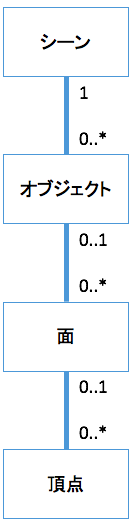
\includegraphics[scale=0.5]{images/er}
    \caption{データモデル間の依存関係}
    \label{データ構造}
  \end{center}
\end{figure}
図\ref{データ構造}のようにシーンのデータはオブジェクトを, オブジェクトは面を, 面は頂点をそれぞれ子にもつ. また, 子のみが親の参照先をもつ.

各データのパラメータを図\ref{プロパティ}に示す.
\begin{figure}[htbp]
  \begin{center}
    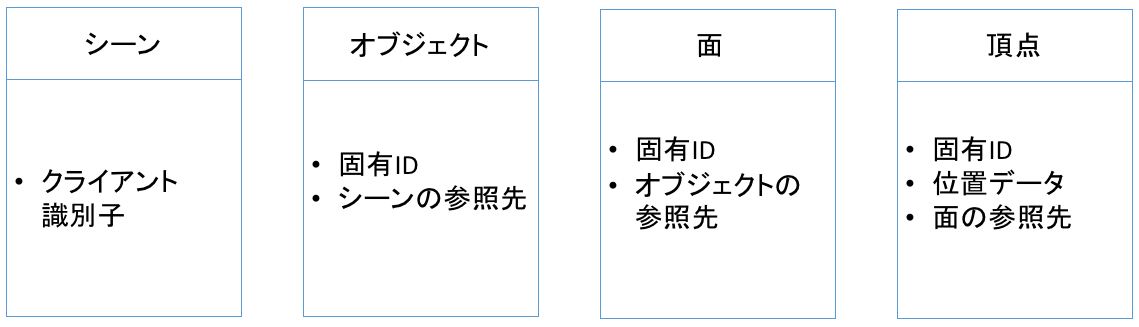
\includegraphics[scale=0.3]{images/prop}
    \caption{データのプロパティ}
    \label{プロパティ}
  \end{center}
\end{figure}
シーンはクライアント識別子というプロパティを持ちサーバシャドウの役割を担う.
またシーンのクライアント識別子に0を与えサーバデータとする.
このデータ構造によって, 子を削除した場合に親との依存関係も削除できる.親を新しく設定する場合, 子のデータを複製しながらそれぞれに新しく設定する親を参照先に設定する.
子のデータを複製していくことによって, 関係を削除した際も複製元のデータは残る.
%%%%%%%%%%%%%%%%%%%%%%%%%%%%%%%%%%
%    固有IDの付与
%%%%%%%%%%%%%%%%%%%%%%%%%%%%%%%%%%
\section{固有IDの付与} \label{固有id}
各データには, 複数クライアント間でIDの衝突が起こるのを防ぐため, そのデータを作成したクライアント識別子を組み込んだ固有IDを与える.
本システムでは図\ref{uuid}のように, クライアント識別子--データモデル識別子--インクリメント番号--ランダム文字列の順につなげた固有IDを与える. クライアント識別子は1から順に振られたユーザIDを用いてクライアントが付与する. また, データモデル識別子は, オブジェクトが0, 面は1, 頂点は2となるように与える.
インクリメント番号は, サーバでもクライアントでも作ったデータの数を記憶しておき, 作るごとにインクリメントする番号である. ランダム文字列は3桁の数字またはアルファベットからなる文字列であり, 固有IDの強豪の発生を抑制する.
\begin{figure}[htbp]
  \begin{center}
    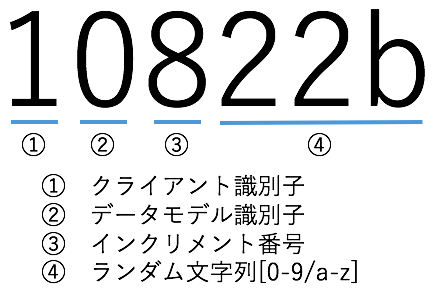
\includegraphics[scale=0.5]{images/uuid}
    \caption{本システムの固有ID}
    \label{uuid}
  \end{center}
\end{figure}
%%%%%%%%%%%%%%%%%%%%%%%%%%%%%%%%%%
%    同期の手順
%%%%%%%%%%%%%%%%%%%%%%%%%%%%%%%%%%
\section{同期の手順}
同期はDifferential Synchronizationに基づいて行う.
同期の手順を具体的な例を用いて説明する. クライアントAは新しく頂点``122xyz''
を作成し, その後, クライアントBは既にある頂点``121abc''を削除する.
クライアントAの同期の手順を図\ref{sycle1}に示す.
クライアントAが編集を行うと, クライアントAのクライアントデータに``122xyz''が作成される(図\ref{sycle1}(a)).
また, 一定時間ごとに同期の処理を行う. クライアントAでは, 差分を計算し, [+ ``122xyz'']となる. [+ ``122xyz'']をクライアントAのサーバシャドウと, サーバデータに適用する(図\ref{sycle1}(b)). その時クライアントAではクライアントデータをクライアントシャドウにシャドウコピーする(図\ref{sycle1}(c)). サーバでは差分を計算し, 差分なし[ ]となる(図\ref{sycle1}(d)). この際にサーバではサーバデータをクライアントAのサーバシャドウにシャドウコピーする(図\ref{sycle1}(e)).
クライアントBの同期の手順を図\ref{sycle2}に示す.
クライアントBが編集を行うと, クライアントBのクライアントデータにある``121abc''を削除する(図\ref{sycle2}(a)).
また, クライアントAと同様に一定時間ごとに同期の処理を行う. 差分を計算し, [-- ``121abc'']となる. [-- ``121abc'']をクライアントBのサーバシャドウと, サーバデータに適用する(図\ref{sycle2}(b)). その時クライアントBではシャドウコピーする(図\ref{sycle2}(c)). サーバでは差分を計算し, [+ ``122xyz'']となる. [+ ``122xyz'']をクライアントBのクライアントデータとクライアントシャドウに適用する(図\ref{sycle2}(d)). この際にサーバではシャドウコピーする(図\ref{sycle2}(e)).
またクライアントBの編集をクライアントAが検知して, 各クライアント間でデータが一致するまでの手順を図\ref{sycle3}に示す.
まず, クライアントAが差分を計算し差分なし[ ]となる(図\ref{sycle3}(a)).
差分なし[ ]なので, サーバデータとサーバシャドウに適用するものはない(図\ref{sycle3}(b)), その時クライアントAではシャドウコピーを行う(図\ref{sycle2}(c)).
次に, サーバデータとサーバシャドウの差分を計算し,  [-- ``121abc'']となる\ref{sycle3}(d)). [-- ``121abc'']をクライアントAのクライアントデータとクライアントシャドウに適用する.
この手順により各クライアントのクライアントデータ, クライアントシャドウ, サーバのサーバデータとサーバシャドウのデータが一致し, 同期が可能となる.
\par
本来, 変数v1を変数v2にシャドウコピーするならばv2 = v1のように代入することで実装する. しかし, 本システムではデータをデータベースに登録して管理しており, 単純な代入で処理できない.
また, 元のデータを削除し新しくシャドウコピーを作成する方法は, 頻繁にシャドウコピーを行うDifferential Synchronizationでは,
データベースのDELETE命令とCREATE命令を頻発させることになり, 処理においてボトルネックとなってしまう. サーバでのシャドウコピーは, サーバデータとサーバシャドウの差分を取り, サーバシャドウに適用することによって解決する.
\begin{figure}[htbp]
  \begin{center}
    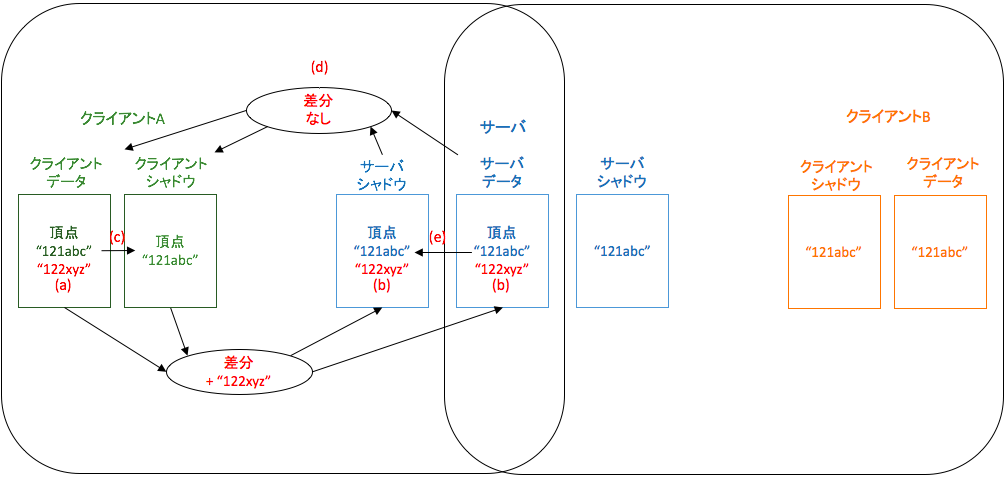
\includegraphics[scale=0.45]{images/sycle1}
    \caption{クライアントAの同期の手順}
    \label{sycle1}
  \end{center}
\end{figure}
\begin{figure}[htbp]
  \begin{center}
    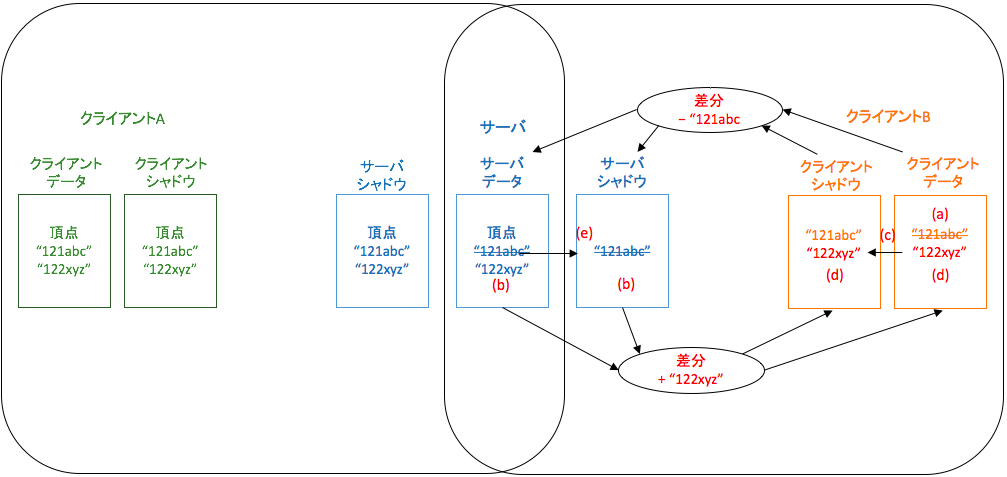
\includegraphics[scale=0.45]{images/sycle2}
    \caption{クライアントBの同期の手順}
    \label{sycle2}
  \end{center}
\end{figure}
\begin{figure}[htbp]
  \begin{center}
    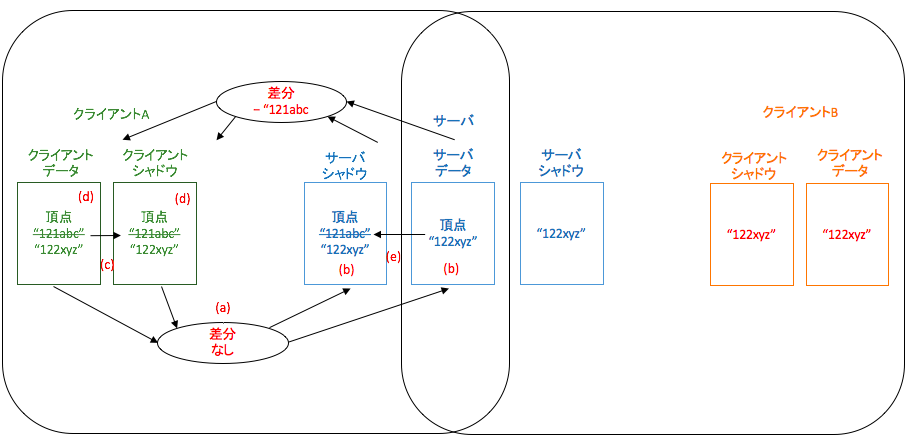
\includegraphics[scale=0.5]{images/sycle3}
    \caption{2回目のクライアントAの同期の手順}
    \label{sycle3}
  \end{center}
\end{figure}
%%%%%%%%%%%%%%%%%%%%%%%%%%%%%%%%%%
%    基本命令
%%%%%%%%%%%%%%%%%%%%%%%%%%%%%%%%%%
\section{基本命令} \label{ope}
オブジェクト, 面, 頂点の各データモデルに対して, 作成, 親への参照の追加, 削除の3つの基本命令を定義する.
基本命令はシステムに対する最低限の命令であり, これらの命令を組み合わせることで, 3Dモデリングで使われる面の分割や押し出しなど, より高度な命令を実現できる.
作成の命令を適用する際のデータの変化を図を用いて説明する.
まず最初のデータとして図\ref{命令0}のように, 面が1つ, 頂点が2つあり, 一方の頂点が面を参照しているとする.
\begin{figure}[htbp]
  \begin{center}
    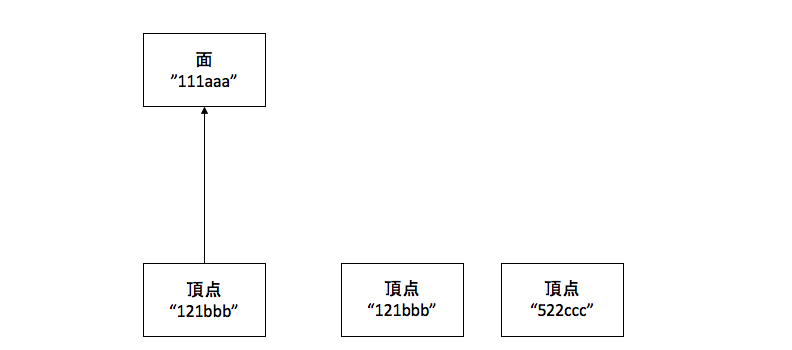
\includegraphics[scale=0.45]{images/ope0}
    \caption{最初のデータ}
    \label{命令0}
  \end{center}
\end{figure}
図\ref{命令0}のデータに対して, 頂点の作成命令を適用した場合のデータの変化を図\ref{命令1}に示す. 図\ref{命令1}では頂点``123ddd''を作成した.
\begin{figure}[htbp]
  \begin{center}
    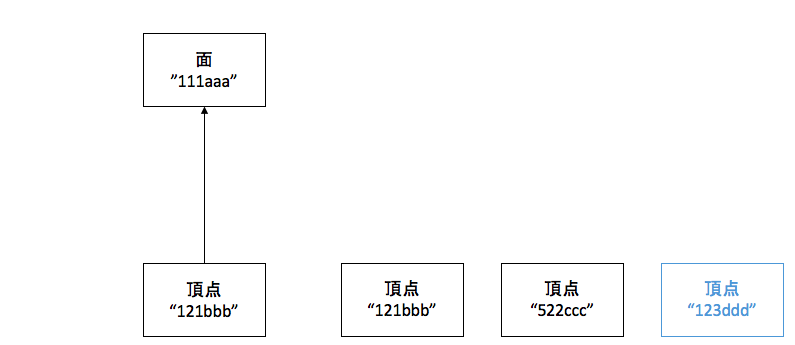
\includegraphics[scale=0.45]{images/ope1}
    \caption{作成命令適用後}
    \label{命令1}
  \end{center}
\end{figure}
図\ref{命令1}のデータである頂点``522ccc''に対して, 面``111aaa''を親とする参照の追加命令を適用した場合のデータの変化を図\ref{命令2}に示す. 図\ref{命令2}では子である頂点``522ccc''を複製しながら面への参照をする.
\begin{figure}[htbp]
  \begin{center}
    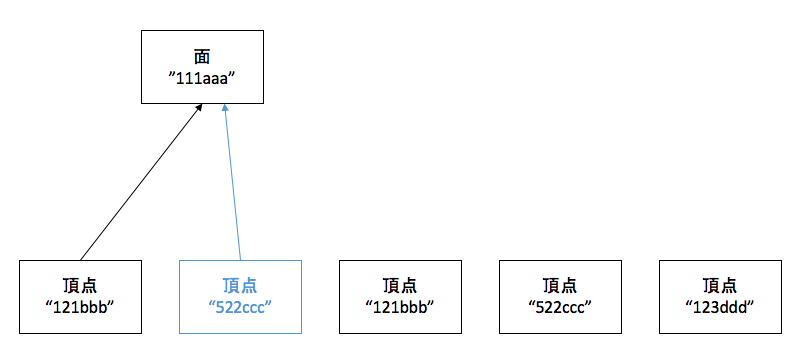
\includegraphics[scale=0.45]{images/ope2}
    \caption{親への参照追加命令適用後}
    \label{命令2}
  \end{center}
\end{figure}
図\ref{命令2}のデータである頂点``123ddd''に対して, 削除命令を適用した場合のデータの変化を図\ref{命令3}に示す. 図\ref{命令3}では, 頂点``123ddd''が削除される.
\begin{figure}[htbp]
  \begin{center}
    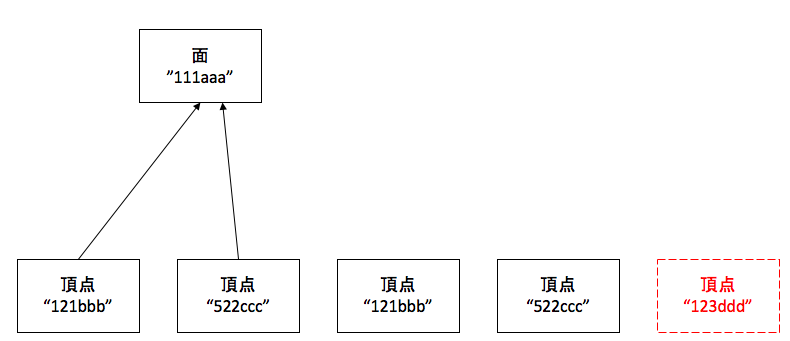
\includegraphics[scale=0.45]{images/ope3}
    \caption{削除命令適用後}
    \label{命令3}
  \end{center}
\end{figure}
図\ref{命令3}のデータである頂点``522ccc''に対して, 削除命令を適用した場合のデータの変化を図\ref{命令4}に示す. 図\ref{命令4}では, 頂点``522ccc''であるデータが複数あるが, 全ての 頂点``522ccc''に関するデータを削除する. この際に, 子が親の参照先を持っているので, 参照関係も同時に消える.
\begin{figure}[htbp]
  \begin{center}
    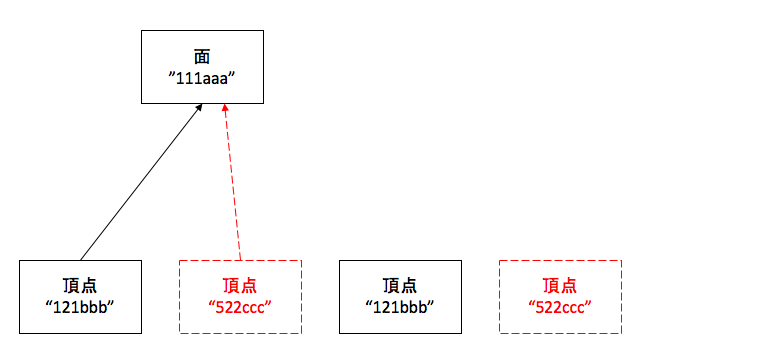
\includegraphics[scale=0.45]{images/ope4}
    \caption{参照関係を含んだデータの削除命令適用後}
    \label{命令4}
  \end{center}
\end{figure}
図\ref{命令4}のデータである面``111aaa''に対して, 削除命令を適用した場合のデータの変化を図\ref{命令5}に示す. 図\ref{命令5}では, 面``111aaa''が削除され, それを参照している子のデータも一緒に削除する. この際, 参照がないデータは削除されない.
\begin{figure}[htbp]
  \begin{center}
    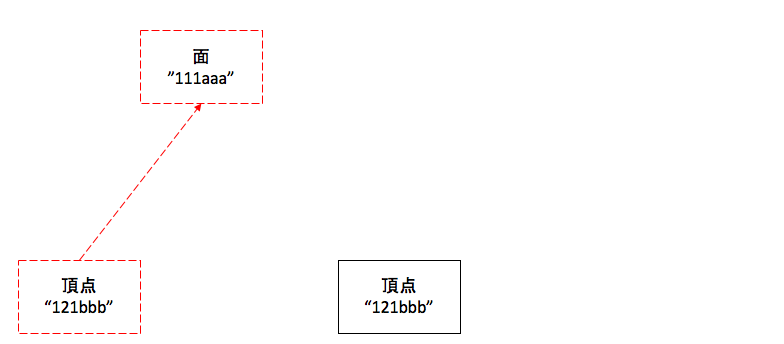
\includegraphics[scale=0.45]{images/ope5}
    \caption{親のデータの削除命令適用後}
    \label{命令5}
  \end{center}
\end{figure}
削除命令や親への参照の追加をする命令を適用する際, 命令の対象がない場合は適用を無効とする.
